%!TeX root=../tese.tex
%("dica" para o editor de texto: este arquivo é parte de um documento maior)
% para saber mais: https://tex.stackexchange.com/q/78101/183146

%% ------------------------------------------------------------------------- %%
\chapter{Implementação do Projeto}
\label{cap:Implementação}

Agora que foram definidas as mecânicas de jogo do ponto de vista de um jogador e
explicado que uma das intenções do projeto é facilitar o aprendizado de um 
iniciante em computação é preciso explicar melhor os detalhes da implementação
para concluir a segunda intenção do projeto que é permitir a extensão do jogo
por alguém que já conheça um pouco de programação ou esteja interessado em 
modificar o código fonte, inserindo novas funcionalidades. 

Para isso, essa seção divide a explicação dos arquivos do jogo agrupando por 
funcionalidades, assim entender o código de implementação torna-se mais simples.

\section{Inventário}

Dentro dos arquivos do jogo (diretório \textit{Phoenix Rising}) é encontrado na 
pasta \textit{GenericGameScenes} e administra os comandos disponíveis e a
movimentação deles na tela.

A seguir estão imagens com os nós que compõem a cena, os métodos do script
atrelado ao nó raiz, chamado \textit{Inventory} e as variáveis mais importantes
para entender o código.

\begin{minipage}[c]{0.5\textwidth}
    \begin{figure}[H]
        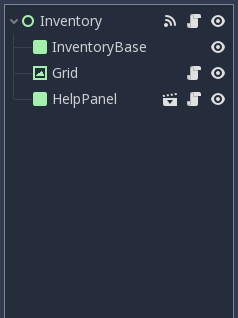
\includegraphics[scale=0.6]{../figuras/cena_inventory.png}
        \caption{Árvore da cena Inventory}
    \end{figure}
\end{minipage}%
\begin{minipage}[c]{0.5\textwidth}
    \begin{figure}[H]
        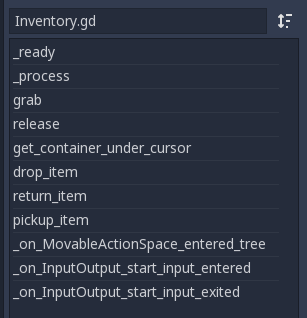
\includegraphics[scale=0.6]{../figuras/funcoes_inventory.png}
        \caption{Funções do script do nó Inventory}
    \end{figure}
\end{minipage}

\begin{figure}[H]
    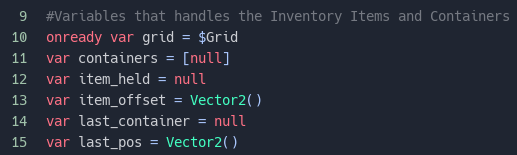
\includegraphics[scale=0.7]{../figuras/variaveis_inventory.png}
    \caption{Variáveis do script do nó Inventory}
\end{figure}

O nó \textit{InventoryBase} apenas dá cor ao espaço destinado aos comandos no
início do jogo e o nó \textit{HelpPanel} é uma cena instanciada que gerencia o
menu de ajuda que aparece ao solicitar mais explicações sobre um comando.

Dentro do jogo \textit{Phoenix Rising} os comandos disponíveis devem ocupar o
espaço de áreas específicas. Estas áreas são chamadas de recipientes (do 
inglês \textit{container}). Um recipiente pode ser o próprio \textit{Grid} do 
inventário ou espaços definidos dentro dos Espaços de Ação, que serão explicados
posteriormente.

O nó \textit{Grid} tem grande importância dentro da cena, pois é ele quem separa
cada recipiente da tela de jogo em pequenos quadradinhos, facilitando a mecânica
de mover os comandos disponíveis. Estes recipientes são adicionados na lista de 
\textit{containers}, definida na linha 11 da figura 3.3.

Para facilitar o entendimento, veja as variáveis mais importantes e o método de 
inicialização da grade (do inglês \textit{grid}):

\begin{minipage}[c]{0.5\textwidth}
    \begin{figure}[H]
        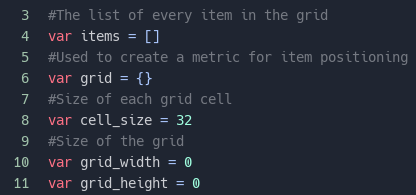
\includegraphics[scale=0.5]{../figuras/grid_variables.png}
        \caption{Variáveis do Grid}
    \end{figure}
\end{minipage}%
\begin{minipage}[c]{0.6\textwidth}
    \begin{figure}[H]
        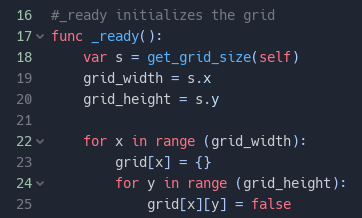
\includegraphics[scale=0.6]{../figuras/grid_ini.png}
        \caption{inicialização do Grid}
    \end{figure}
\end{minipage}

O tamanho de cada quadrado é armazenado e definido na linha 8 da figura 3.4
e as medidas da grade são armazenadas pelas variáveis definidas nas linhas
10 e 11 da mesma figura.

Na inicialização da grade do inventário o método \textit{get\_grid\_size} 
recebe o retângulo que foi definido para ser o recipiente e devolve seu 
tamanho (largura e altura) usando o sistema quadriculado, ou seja, devolve 
quantos quadrados de largura e altura ele ocupa. Depois, cada posição 
desta grade recebe o valor "falso", sinalizando que aquele quadrado está vazio,
ou seja, que nenhum item do jogo ocupa aquelas posições.

A partir dessa divisão todo comando que é disponibilizado no inventário ocupará
um número de quadrados do \textit{grid} e a movimentação destes itens é feita 
pelos métodos de pegar (do inglês \textit{grab}) e soltar (do inglês 
\textit{release}) definidos no \textit{scripts} do nó \textit{Inventory}. Ao
posicionar um comando em alguma região do recipiente os quadrados são marcados
com "verdadeiro" para sinalizar que aquela região está preenchida.

\begin{figure}[H]
    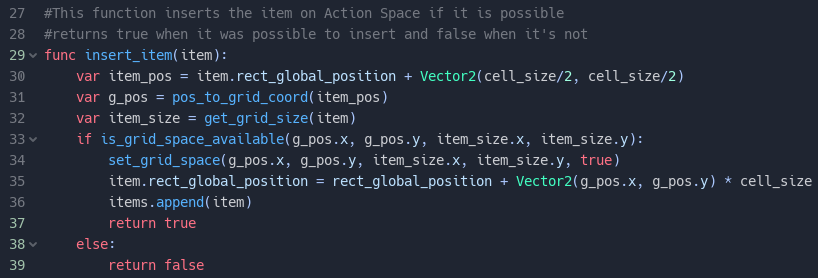
\includegraphics[scale=0.6]{../figuras/insere_item.png}
    \caption{Método de inserção de um item}
\end{figure}

\begin{figure}[H]
    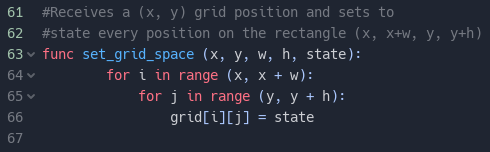
\includegraphics[scale=0.7]{../figuras/marca_grid.png}
    \caption{Marcação das posições do grid}
\end{figure}

\section{Espaço de Ação}

Dentro dos arquivos do jogo (diretório \textit{Phoenix Rising}) é encontrado na 
pasta \textit{ActionSpace}

\section{Processo Visual}

Dentro dos arquivos do jogo (diretório \textit{Phoenix Rising}) é encontrado na
pasta \textit{VisualProcess}

\section{Nível Base}

Dentro dos arquivos do jogo (diretório \textit{Phoenix Rising}) é encontrado na
pasta \textit{BaseLevel}

\section{Cenas Genéricas}

Dentro dos arquivos do jogo (diretório \textit{Phoenix Rising}) é encontrado na
pasta \textit{GenericGameScenes}

\section{Comportamento dos Comandos}

Dentro dos arquivos do jogo (diretório \textit{Phoenix Rising}) é encontrado na
pasta \textit{RunEnvironment}

\section{Cenas de Execução}

Dentro dos arquivos do jogo (diretório \textit{Phoenix Rising}) é encontrado na
pasta \textit{RunEnvironment}

\section{Ajuda ao Usuário}

Dentro dos arquivos do jogo (diretório \textit{Phoenix Rising}) é encontrado na
pastas \textit{UsersGuide} e em \textit{GenericGameScenes} 



